%
% $RCSfile: module_modelling.tex,v $
%
% Copyright (C) 2002-2008. Christian Heller.
%
% Permission is granted to copy, distribute and/or modify this document
% under the terms of the GNU Free Documentation License, Version 1.1 or
% any later version published by the Free Software Foundation; with no
% Invariant Sections, with no Front-Cover Texts and with no Back-Cover
% Texts. A copy of the license is included in the section entitled
% "GNU Free Documentation License".
%
% http://www.cybop.net
% - Cybernetics Oriented Programming -
%
% http://www.resmedicinae.org
% - Information in Medicine -
%
% Version: $Revision: 1.1 $ $Date: 2008-08-19 20:41:07 $ $Author: christian $
% Authors: Christian Heller <christian.heller@tuxtax.de>
%

\subsection{Module Modelling}
\label{module_modelling_heading}
\index{CYBOL}
\index{Programming Language}
\index{Electronic Health Record}
\index{EHR}
\index{Web User Interface}
\index{WUI}
\index{Hyper Text Markup Language}
\index{HTML}
\index{User Interface}
\index{UI}
\index{Ontology}
\index{Translator Pattern}
\index{Looping}

When CYBOI had become more stable (besides the extensions that were -- and are
-- frequently implemented), development could focus on the actual application
again. From now on, \emph{Res Medicinae} modules only had to be \emph{modelled}
in CYBOL, but no longer had to be \emph{coded} in a programming language. The
designed state- and logic knowledge, existing in form of CYBOL templates,
already represented the complete application; no further implementation phase
was needed.

\begin{figure}[ht]
    \begin{center}
        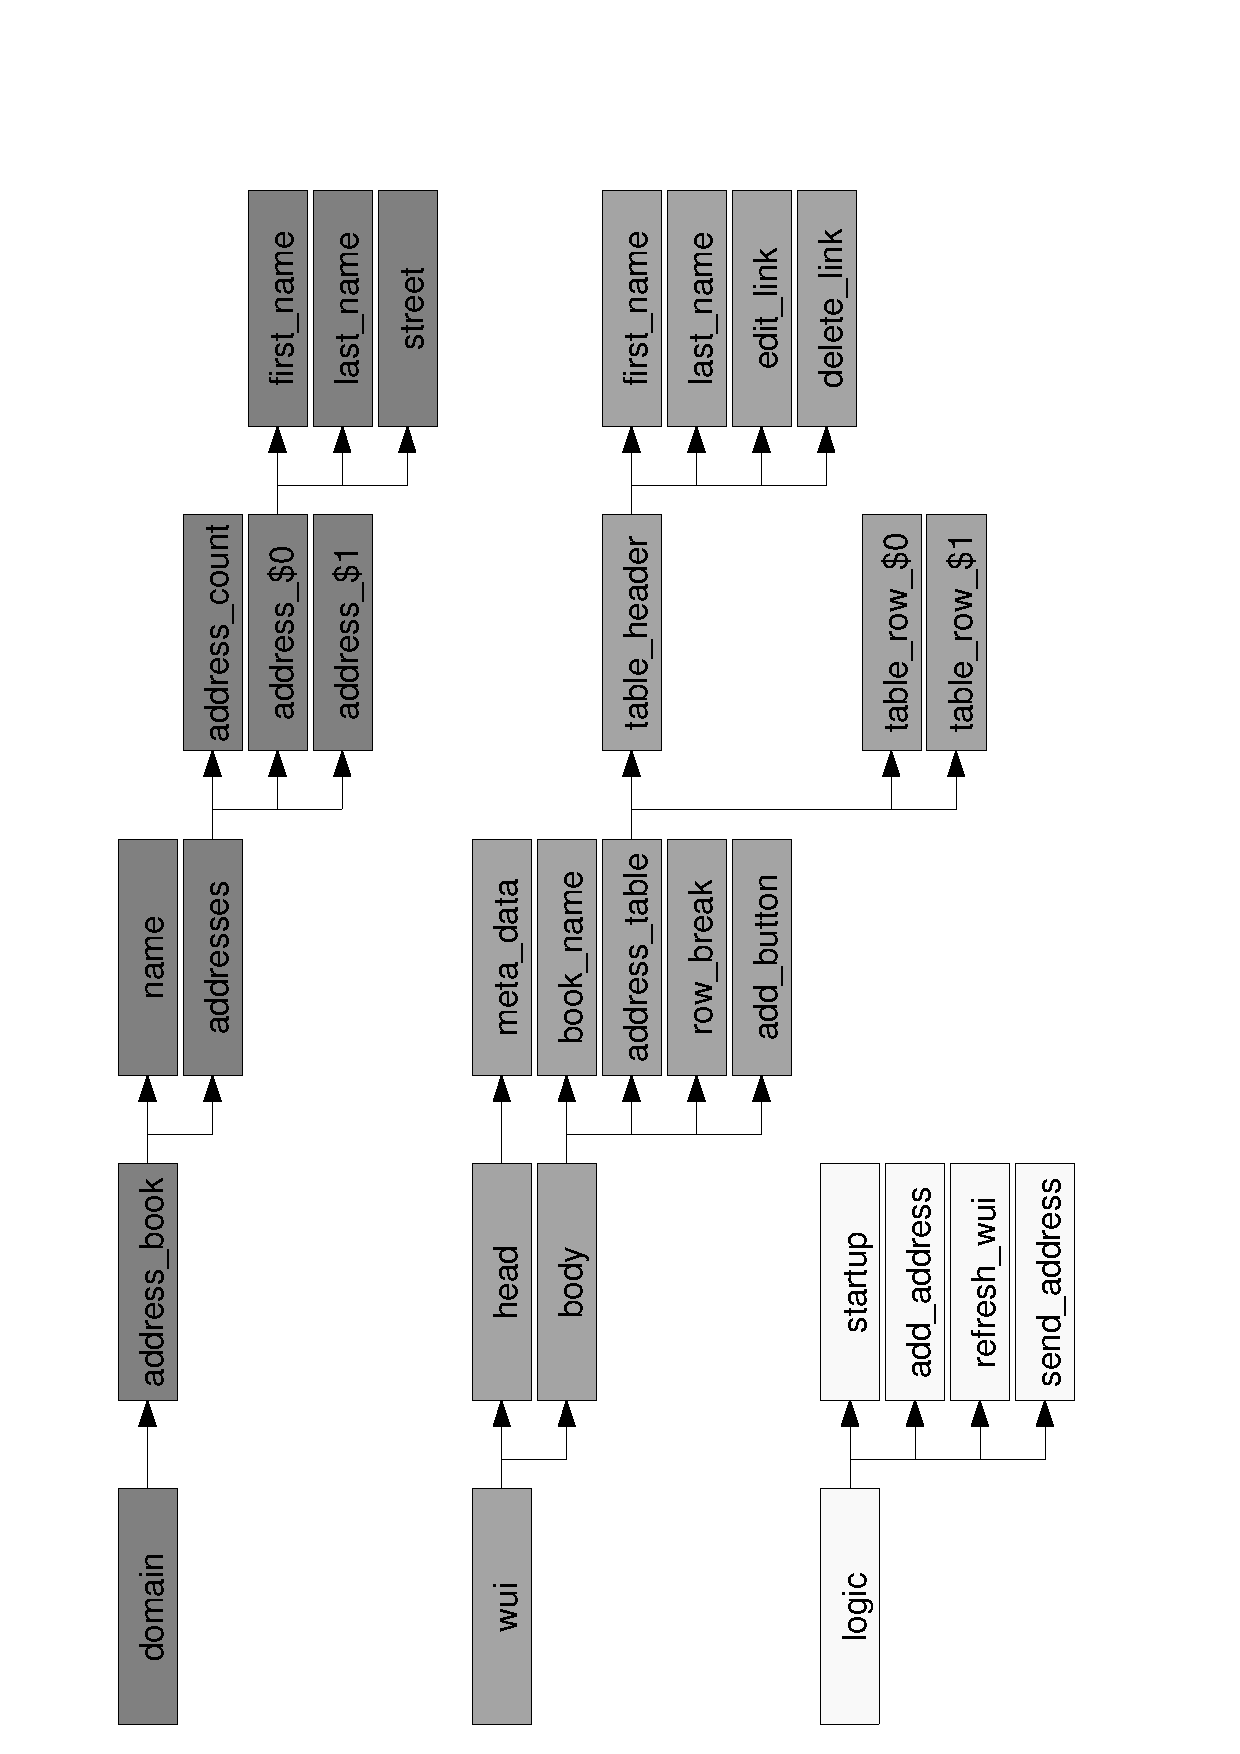
\includegraphics[scale=0.3,angle=-90]{graphic/radesign.pdf}
        \caption{ResAdmin Knowledge Models (Extract)}
        \label{radesign_figure}
    \end{center}
\end{figure}

Due to the tremendous complexity of an \emph{Electronic Health Record} (EHR),
only a very small part of its data could be considered for the application
prototype within this work. Administrative data like a person's name or address
are standard information found in all EHRs. A corresponding module named
\emph{ResAdmin} \cite{holzmueller2005} was therefore elected to be realised
first (compare module list in section \ref{core_model_heading}). Its models
belong to three categories: \emph{Domain}, \emph{Web User Interface} (WUI) and
\emph{Logic} (figure \ref{radesign_figure}).

\begin{figure}[ht]
    \begin{center}
        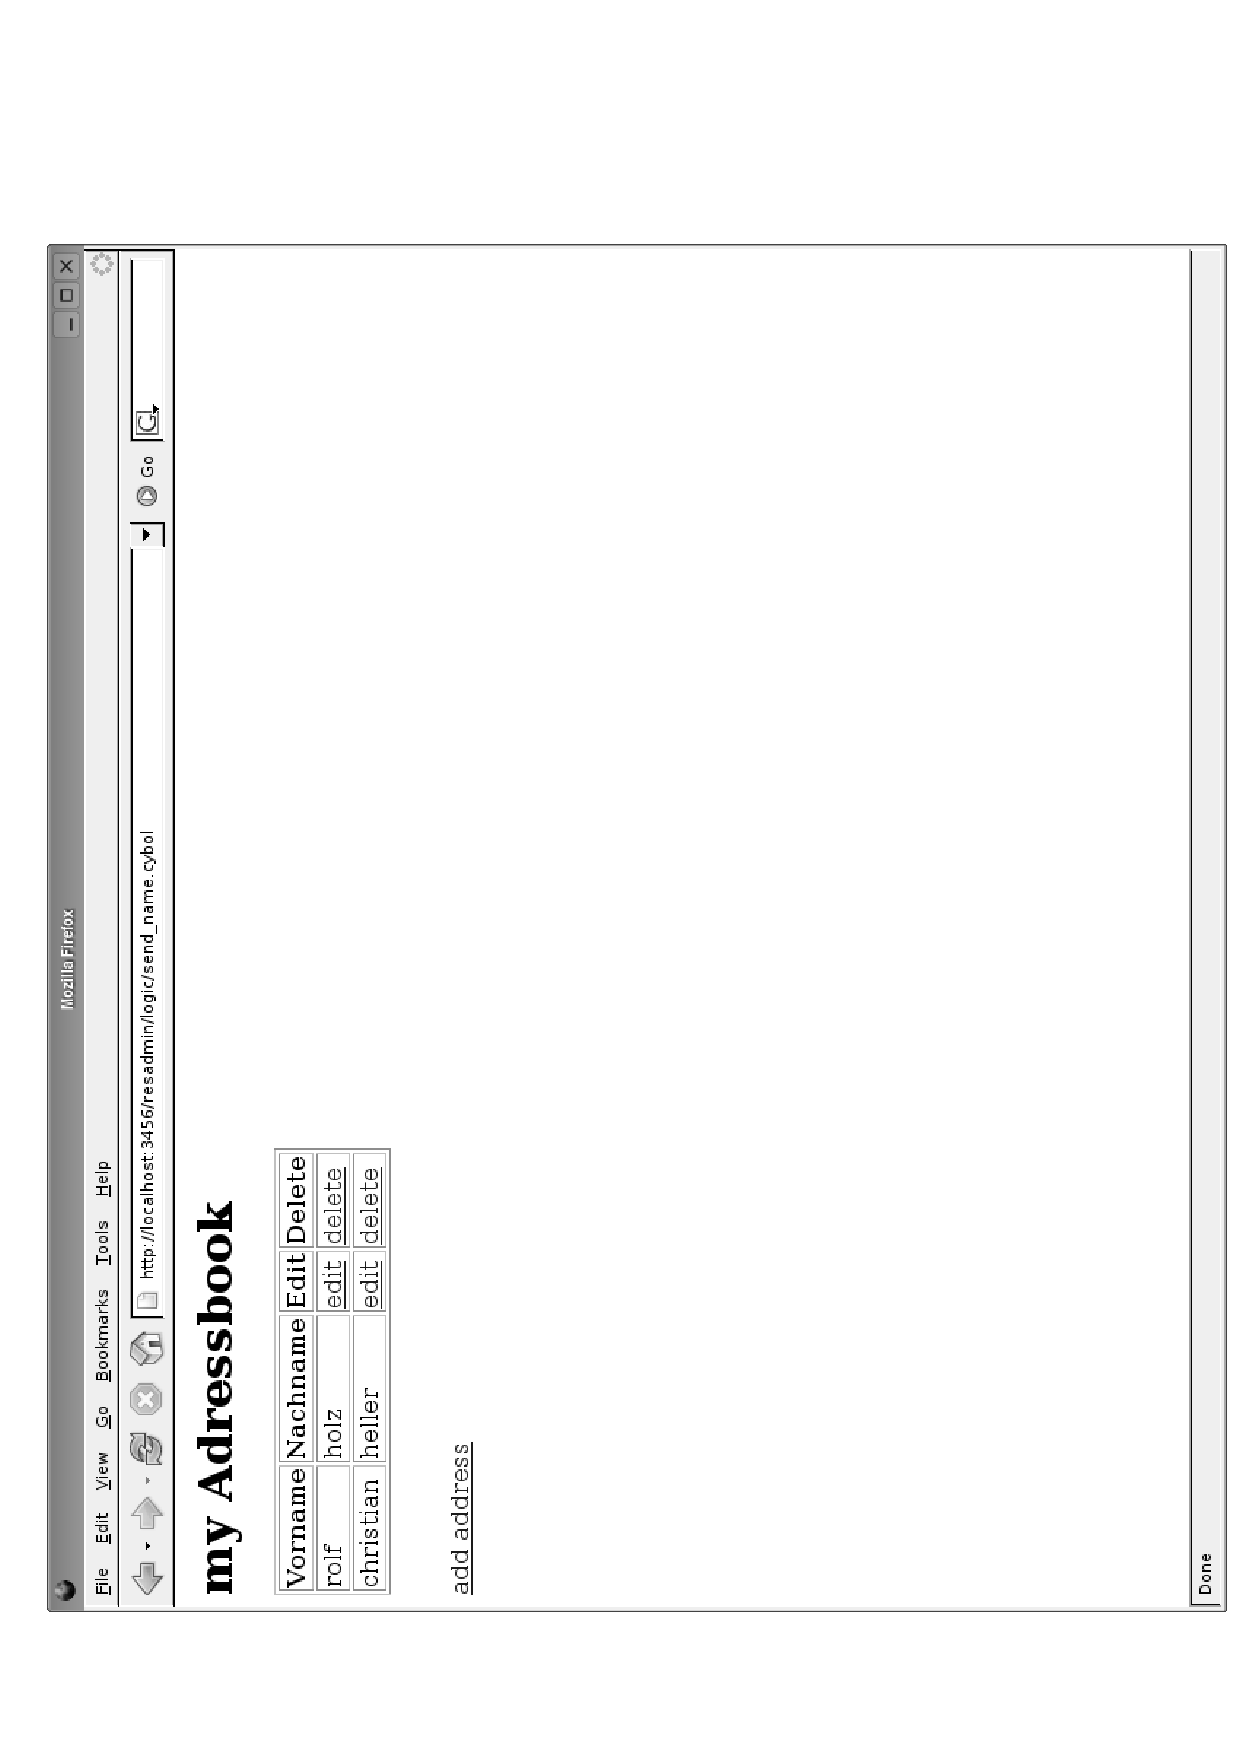
\includegraphics[scale=0.3,angle=-90]{graphic/resadmin.pdf}
        \caption{Simple Web User Interface of the ResAdmin Module \cite{holzmueller2005}}
        \label{resadmin_figure}
    \end{center}
\end{figure}

The addresses contained in the \emph{domain} branch of the knowledge tree are
manipulated across \emph{Hyper Text Markup Language} (HTML) \emph{User Interface}
(UI) models belonging to the \emph{web} branch of that same tree. An example
structure of a knowledge tree was shown in figure \ref{mvctree_figure}. Figure
\ref{resadmin_figure} shows the minimal WUI. Every action model that a user can
trigger through the WUI exists as part of the \emph{logic} branch of the
knowledge tree.

Independently of what kind of knowledge model (state or logic) was created, the
ontological principles (section \ref{knowledge_representation_heading}) were
strictly followed. Most importantly, relations within a hierarchical model were
always \emph{unidirectional}, that is from a \emph{Whole-} to its \emph{Part}
models, but never the other way around. Additionally, however, logic models may
reference and access runtime state models.

Some of the logic models represent \emph{Translators} (compare section
\ref{translator_architecture_heading}). They extract address information
residing in the domain- and copy them to the web model, which is afterwards
sent to the human user as communication partner. This principle holds true for
the communication between application systems, only that then other than web
models are used as communication format. The vision to make all communication
channels really \emph{transparent} and easy to handle for the user now seems to
be coming true. The following example shows an extract of a CYBOL logic
knowledge template for ResAdmin:

\begin{scriptsize}
    \begin{verbatim}
<part name="set_loop_index" channel="inline" abstraction="operation" model="copy">
    <property name="source" channel="inline" abstraction="integer" model="0"/>
    <property name="destination" channel="inline" abstraction="knowledge"
        model="domain.index"/>
</part>
<part name="set_address_count" channel="inline" abstraction="operation" model="count_parts">
    <property name="basename" channel="inline" abstraction="string" model="address"/>
    <property name="model" channel="inline" abstraction="knowledge"
        model="domain.addressbook.addresses"/>
    <property name="result" channel="inline" abstraction="knowledge"
        model="domain.addressbook.addresses.address_count"/>
</part>
<part name="compare" channel="inline" abstraction="operation" model="compare">
    <property name="left_operand" channel="inline" abstraction="knowledge"
        model="domain.index"/>
    <property name="right_operand" channel="inline" abstraction="knowledge"
        model="domain.addressbook.addresses.address_count"/>
    <property name="operator" channel="inline" abstraction="string"
        model="greater_or_equal"/>
    <property name="result" channel="inline" abstraction="knowledge"
        model="domain.break_flag"/>
</part>
<part name="create_table_body" channel="inline" abstraction="operation" model="loop">
    <property name="break" channel="inline" abstraction="knowledge"
        model="domain.break_flag"/>
    <property name="index" channel="inline" abstraction="knowledge"
        model="domain.index"/>
    <property name="model" channel="inline" abstraction="knowledge"
        model="logic.create_table_rows"/>
</part>
<part name="send_wui" channel="inline" abstraction="operation" model="send">
    <property name="language" channel="inline" abstraction="string" model="tcp_socket"/>
    <property name="receiver" channel="inline" abstraction="string" model="user"/>
    <property name="message" channel="inline" abstraction="knowledge" model="web"/>
</part>
    \end{verbatim}
\end{scriptsize}

The loop \emph{index} and \emph{address\_count} parameters are initialised
first, before a comparison operation possibly sets the loop's
\emph{break\_flag}. Then, the actual loop is executed and table rows are
created, until the break flag is really set. Finally, the complete \emph{web}
knowledge model is sent via \emph{tcp\_socket} to the human \emph{user} as
receiver watching the WUI graphically rendered by a web browser.

It can be concluded that the simple prototype module \emph{ResAdmin}, realised
within the \emph{Res Medicinae} project, demonstrates how a CYBOL application
including domain-, user interface- and logic models may look like.
